% Paste-ready fragment converted from ``Jimmy Final Draft.docx``.
% Preamble addition required by this fragment: \usepackage{longtable} (graphicx is already used by main.tex).

\section{Research question and variables}
The independent variable is the distance between the slit and the screen and will include values thatrange from the [nearby and further apart]. The [nearby] will include 20cm, 40cm, 60cm, 80cm, and 100cm while the further apartinclude 3 meters, 5 meters, 6 meters, and 8 meters.

Since the fringe spacing is within the milimeter range and itis beyond my human ability to hold the clipboard still within milimeter stillness while using the other hand to hold a pencil and mark accurately on the paper live. I decided to take a high resolution photo ofthe projection on a graphed piece of paper as a photo is most versatile and captures exactly as seen. The graphed piece of paper is printed with milimeter accuracy markings. as a resultI will measure distance between each adjacentfringe (in milimeters) with software solutions and excuse my skill issue.

\textbf{Research question.} What is the relationship with the distance between screen and slit (from the range of 20cm to 8m) and the spacing between adjacent bright fringes (in mm) in a double slit system.

\section{Background}
Wave phenomena states that wave could interfere when they overlap. When two waves are in opposite phase, itis said to interfere destructively and cancel out. However, ifthey are the same phase and interferes, itis said to be constructive, reaching a greater amplitude.

The debate of whether lightis a particle or a wave was challenged by Thomas Young's famous Double Slit Experimentin Young's Course of Lectures on Natural Philosophy and the Mechanical Arts of1807 , where a coherentlight source shining through two tiny slits projected an interference pattern with alternation between light and dark fringes ratherthan two individual bright fringes in a dark background. The formula proposed by Thomas Young was

\begin{equation} s = \frac{\lambda D}{d} \end{equation}
In which ``S'' is the distance between two adjacent brightfringes, \ensuremath{\lambda} is wavelength ofthe light, D is the distance between the screen and slits in meters and d is the distance between slits.

The mathematical undergirding is as thus justified[4]:

Engage thy eyes upon the following graph:

We observe thatthe path difference from the wave from the bottom slit and top slitis illustrated as \ensuremath{\Delta}x,this coincides with the equation

\begin{equation} d\sin\theta=\Delta x \end{equation}
(pls Ms. Cupp make these equations smallerthx). We observe the factthatthe path difference (\ensuremath{\Delta}x)for constructive waves is

\begin{equation} n\lambda \end{equation}
where \ensuremath{\lambda} is the wavelength ofthe light and n is an integer representing the interested brightfringe.

\section{Experimental design}
\begin{longtable}{p{0.29\linewidth}p{0.34\linewidth}p{0.29\linewidth}}
\caption{Variables, methods, and justifications}\label{tab:variables}\\
\hline
Independent variable & Method of how this variable will be changed & Justification: Why this range, interval or frequency was chosen? \\
\hline
Distance between Slit and screen & Forthe long range,there will be three objects the pattern will be projected on,the object chosen is a graphed piece of paper on a clipboard, suspended hanging on a table. For each distance, the source will move between 3 distances, and once the data for each table is collected, it will be moved away to revealthe nexttable. For the shortrange data, the projected screen will move on a wheel on tracks. & This range of data will provide us justification for not only the short range, but also long range to show the validity ofthe double slit equation over a range of distances. \\
Dependent Variable & Method of how this variable will be measured & Justification: How many trials? How will precise and sufficient data be collected? \\
The distance between adjacentfringes on the projected screen & I willtake a high resolution image with my phone and use perspective correction on the image and use software solutions such as imageJto find the average distance between each fringe & One picture will be taken for each distance.But multiple takes on fringe spacing will be recorded and the average will be found. \\
Control Variable & Potential impacts of this variable on the dependent variable/data & How it will be controlled and kept constant \\
The same laser and slit &  &  \\
same method is used to measure the distances &  &  \\
\hline
\end{longtable}

\section{Data analysis}
Qualitative: I don't recall having taped the paper onto the surface of the clipboard for maximum flatness of the surface

\begin{longtable}{p{0.46\linewidth}p{0.46\linewidth}}
\caption{Qualitative observations and interpretations}\label{tab:qualitative}\\
\hline
Qualitative observations & Interpretations/Photos \\
\hline
I don't recall having taped the paper onto the surface of the clipboard for maximum flatness of the surface. The paper is clipped on the right side but not the left & This means when we do the perspective shifts it might have slight distortions \newline 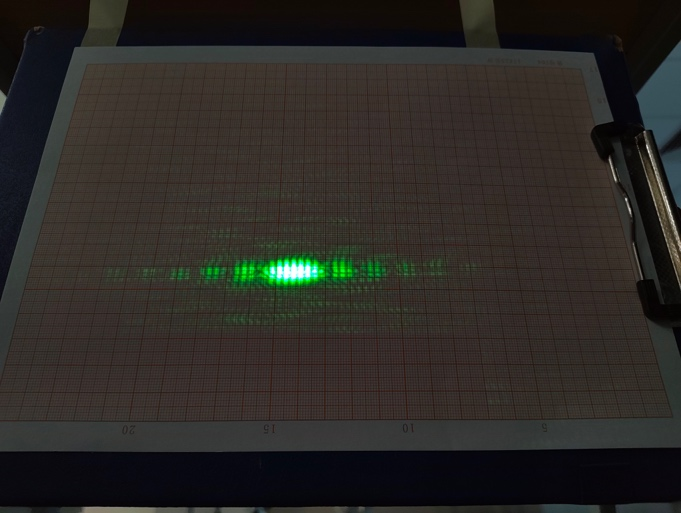
\includegraphics[width=\linewidth]{Images/JimmyDraft/image1.jpeg} \\
Some are really slanted for some reason. I ended up correcting it by drawing lines with respect to the direction of the slant and then measuring with that angle & 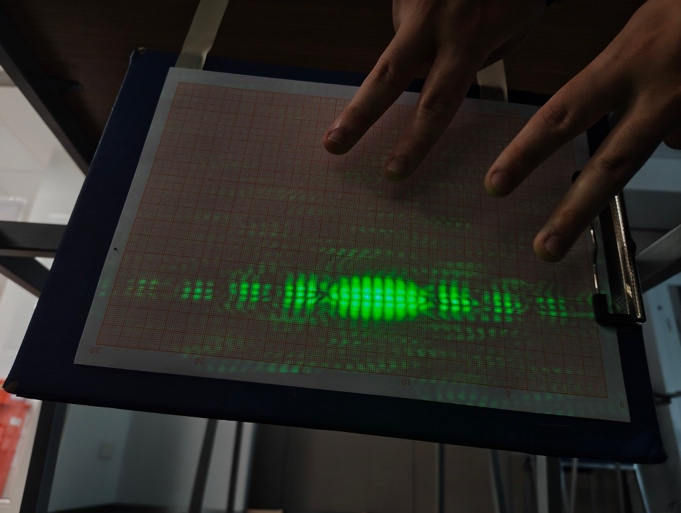
\includegraphics[width=\linewidth]{Images/JimmyDraft/image2.jpeg} \newline 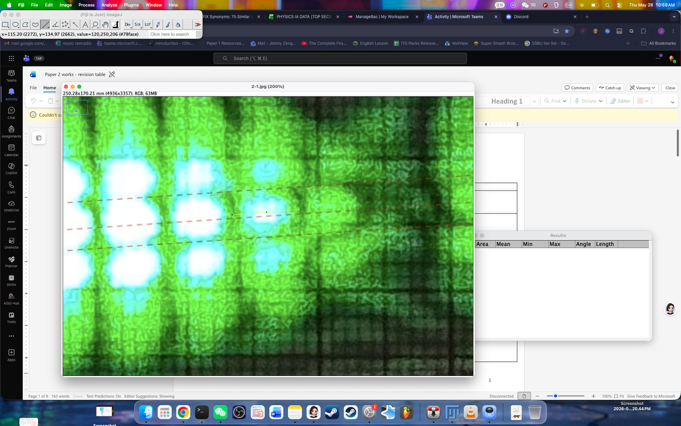
\includegraphics[width=\linewidth]{Images/JimmyDraft/image3.png} \\
Some of the fringes are too unclear to be seen I have noted them in my data when there were issues measuring & 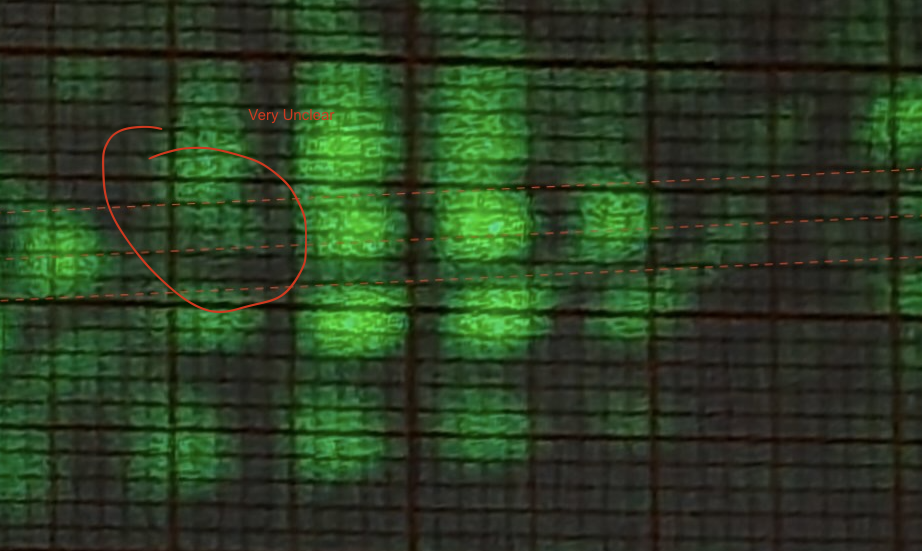
\includegraphics[width=\linewidth]{Images/JimmyDraft/image4.png} \\
There are shadows sometimes in the data. This is also noted & 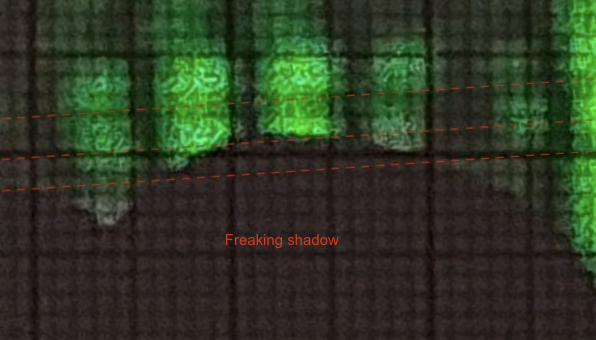
\includegraphics[width=\linewidth]{Images/JimmyDraft/image5.png} \\
\hline
\end{longtable}

\section{Raw and processed measurements}
\begin{longtable}{p{0.28\linewidth}p{0.105\linewidth}p{0.105\linewidth}p{0.105\linewidth}p{0.105\linewidth}p{0.105\linewidth}p{0.105\linewidth}}
\caption{Measurements for data sets 1-1, 1-2, and 1-3}\label{tab:data1}\\
\hline
 & 1-1 &  & 1-2 &  & 1-3 &  \\
\hline
Pixels per cm square side length (pixels/cm). Used as a reference of size. & 334.005 & 332.667 & 149.678 & 150.251 & 149.169 & 150.667 \\
Pixels per cm square side length (pixels/cm). Used as a reference of size. & 323.488 & 329.334 & 151.627 & 151.503 & 150.334 & 153.004 \\
Pixels per cm square side length (pixels/cm). Used as a reference of size. & 332.669 & 332.003 & 154.002 & 149.231 & 150.17 & 149.333 \\
Mean & 330.694 &  & 151.049 &  & 150.4461667 &  \\
Measurement of paper graph square side length after setting the mean (above) as reference & 1.036 & 1.005 & 1.004 & 0.949 & 1.000 & 0.989 \\
Measurement of paper graph square side length after setting the mean (above) as reference & 1.013 & 0.953 & 1.081 & 1.01 & 0.975 & 0.972 \\
Measurement of paper graph square side length after setting the mean (above) as reference & 0.983 &  & 0.977 &  & 1.022 &  \\
Central Maxima (mm). Measured as the distance from the left/right edge of one bright fringe to the left/right edge of an adjacent bright fringe & Left edge & Right Edge & Left edge & Right Edge & Left edge & Right Edge \\
Central Maxima (mm). Measured as the distance from the left/right edge of one bright fringe to the left/right edge of an adjacent bright fringe & 3.044 & 2.822 & 3.078 & 3.509 & 4.254 & 4.188 \\
Central Maxima (mm). Measured as the distance from the left/right edge of one bright fringe to the left/right edge of an adjacent bright fringe & 2.903 & 2.984 & 3.443 & 3.443 & 4.52 & 4.143 \\
Central Maxima (mm). Measured as the distance from the left/right edge of one bright fringe to the left/right edge of an adjacent bright fringe & 3.014 & 2.923 & 3.608 & 3.575 & 4.032 & 4.055 \\
Central Maxima (mm). Measured as the distance from the left/right edge of one bright fringe to the left/right edge of an adjacent bright fringe & 2.863 & 2.903 & 3.542 & 3.525 & 4.165 & 4.143 \\
Central Maxima (mm). Measured as the distance from the left/right edge of one bright fringe to the left/right edge of an adjacent bright fringe & 2.963 & 2.903 & 3.542 & 3.426 & 4.099 & 4.099 \\
Central Maxima (mm). Measured as the distance from the left/right edge of one bright fringe to the left/right edge of an adjacent bright fringe & 2.974 & 2.812 & 3.492 & 3.525 & 4.143 & 4.365 \\
Central Maxima (mm). Measured as the distance from the left/right edge of one bright fringe to the left/right edge of an adjacent bright fringe &  &  & 3.343 & 3.525 & 4.055 & 4.032 \\
Central Maxima (mm). Measured as the distance from the left/right edge of one bright fringe to the left/right edge of an adjacent bright fringe &  &  & 3.542 &  &  &  \\
First Maxima (mm) & 3.014 & 2.792 & 3.343 & 3.409 & 3.9 & 3.966 \\
First Maxima (mm) & 3.105 & 3.095 & 3.492 & 3.36 & 4.365 & 4.099 \\
First Maxima (mm) & 3.064 & 3.054 & 3.542 & 3.227 & 4.431 & 3.811 \\
First Maxima (mm) & 2.974 & 3.155 & 3.492 & 3.906 & 4.232 & 4.055 \\
Second Maxima & 2.933 &  & 3.426 & 3.062 & 4.032 & 3.877 \\
Second Maxima & 2.979 &  & 3.509 & 3.625 & 4.165 & 3.988 \\
Second Maxima & 2.903 &  & 3.294 & 3.707 & 4.032 & 4.032 \\
(Data deemed difficult to measure consistently for the first one) & 2.767 &  & 3.459 & 3.045 & 4.188 & 3.955 \\
(Data deemed difficult to measure consistently for the first one) & 3.22 &  & 3.261 & 3.327 & 4.276 & 4.154 \\
(Data deemed difficult to measure consistently for the first one) & 2.812 &  & 3.095 & 3.757 & 4.121 & 4.104 \\
Average fringe displacement (mm) & 2.96805 &  & 3.4416 &  & 4.119882353 &  \\
Expected/Calculated Value (mm) & 2.9295 &  & 3.521 &  & 4.112 &  \\
Distance between laser and screen (cm) & 247.8 &  & 297.8 &  & 347.8 &  \\
uncertainty of distance between adjacent bright fringes (mm) & \ensuremath{\pm}0.2265 &  & \ensuremath{\pm}0.4305 &  & \ensuremath{\pm}0.3545 &  \\
\hline
\end{longtable}

\begin{longtable}{p{0.11\linewidth}p{0.11\linewidth}p{0.11\linewidth}p{0.11\linewidth}p{0.11\linewidth}p{0.11\linewidth}p{0.11\linewidth}p{0.11\linewidth}}
\caption{Measurements for data sets 2-1, 2-2, 2-3, and 3-1}\label{tab:data2}\\
\hline
2-1 &  & 2-2 &  & 2-3 &  & 3-1 &  \\
\hline
198.668 & 197.333 & 247.335 & 249.668 & 236.513 & 237.334 & 162 & 162.507 \\
196.667 & 198.669 & 248 & 247.337 & 235.675 & 237.51 & 162.501 & 161.757 \\
196.667 & 195.336 & 248.002 & 247 & 225.281 & 229.847 & 157.009 & 161.174 \\
197.223 &  & 247.89 &  & 233.693 &  & 161.158 &  \\
1.014 & 1.031 & 1.059 & 0.968 & 0.999 & 0.956 & 1.003 & 1.034 \\
1.014 & 1.048 & 1.019 & 0.98 & 1.002 & 1.027 & 1.016 & 1.081 \\
0.98 &  & 0.989 &  & 1.038 &  & 1.024 &  \\
Left edge & Right Edge & Left edge & Right Edge & Left edge & Right Edge & Left edge & Right Edge \\
4.91 & 4.322 & 6.102 & 5.866 & 6.994 & 6.262 & 6.144 & 6.408 \\
5.542 & 5.137 & 5.922 & 5.883 & 6.39 & 6.342 & 6.227 & 6.557 \\
5.306 & 5.316 & 6.099 & 5.74 & 6.524 & 6.393 & 6.455 & 6.186 \\
5.129 & 5.219 & 5.839 & 5.901 & 6.436 & 6.601 & 6.599 & 6.517 \\
5.287 & 5.215 & 6.042 & 6.042 & 6.479 & 6.61 & 6.683 & 6.417 \\
5.479 & 5.413 & 5.987 & 5.9 & 6.302 & 6.308 & 6.372 & 6.31 \\
5.186 & 5.262 & 5.984 &  & 6.479 & 6.732 & 6.537 & 6.682 \\
5.108 & 5.371 &  &  &  &  &  &  \\
5.08 & 5.026 & 5.781 & 5.696 & 6.226 & 6.516 & 6.081 & 6.175 \\
5.184 & 5.434 & 6.066 & 6.061 & 6.664 & 6.601 & 6.765 & 6.484 \\
5.592 & 5.339 & 5.957 & 5.826 & 6.863 & 6.617 & 6.548 & 6.298 \\
6.092 & 5.643 & 5.751 & 6.287 & 6.644 & 6.702 & 6.795 & 6.578 \\
bad data &  & only clear data is extracted & only clear data is extracted &  &  & surprisingly consistent & surprisingly consistent \\
4.928 &  & 5.536 & 5.018 & 6.025 & 5.866 & 6.488 & 6.484 \\
5.192 &  & 5.658 & 5.462 & 6.366 & 6.253 & 6.454 & 6.485 \\
5.282 &  & 6.221 & 5.349 & 6.625 & 6.482 &  &  \\
4.834 &  & 5.723 & 5.933 & 6.177 & 6.869 &  &  \\
5.188 &  & 5.597 & 5.823 & 6.174 &  &  &  \\
5.386 &  &  &  &  &  &  &  \\
5.246733333 &  & 5.840387097 &  & 6.468451613 &  & 6.451115385 &  \\
5.294 &  & 5.885 &  & 6.476 &  & 6.476 &  \\
447.8 &  & 497.8 &  & 547.8 &  & 547.8 &  \\
\ensuremath{\pm}0.885 &  & \ensuremath{\pm}0.6345 &  & \ensuremath{\pm}0.564 &  & \ensuremath{\pm}0.357 &  \\
\hline
\end{longtable}

\begin{longtable}{p{0.13\linewidth}p{0.13\linewidth}p{0.13\linewidth}p{0.13\linewidth}p{0.13\linewidth}p{0.13\linewidth}}
\caption{Measurements for data sets 3-2, 3-3, and 4-3}\label{tab:data3}\\
\hline
3-2 &  & 3-3 &  & 4-3 &  \\
\hline
155.766 & 156 & 189.667 & 191.167 & 162.675 & 163.672 \\
154.253 & 154.001 & 192.667 & 191.707 & 162.003 & 160.502 \\
154.002 & 157.851 & 195.668 & 185.783 & 162.5 & 163.773 \\
155.312 &  & 191.11 &  & 162.521 &  \\
0.966 & 1.009 & 1.042 & 1.055 & 0.985 & 0.964 \\
1.073 & 1.095 & 0.985 & 0.977 & 1.077 & 0.995 \\
0.987 &  & 1.008 &  & 1.088 &  \\
Left edge & Right Edge & Left edge & Right Edge & Left edge & Right Edge \\
7.041 & 7.061 & 7.405 & 7.169 & 10.8 & 10.522 \\
6.955 & 6.718 & 7.98 & 7.352 & 10.77 & 10.4 \\
7.17 & 6.954 & 7.884 & 7.68 & 10.43 & 10.774 \\
6.978 & 6.933 & 7.404 & 7.536 & 10.557 & 10.251 \\
7.212 & 6.89 & 7.771 & 7.745 & 10.863 & 10.896 \\
6.89 & 7.064 & 7.692 & 7.378 & 10.687 & 10.493 \\
 &  & 7.536 & 7.956 &  & 10.585 \\
 &  &  & 7.329 &  & 10.773 \\
6.763 & 6.665 & 7.433 & 7.535 & 10.155 & 10.032 \\
7.211 & 7.179 & 7.902 & 7.222 & 10.739 & 10.465 \\
6.826 & 7.471 & 7.43 & 7.536 & 10.28 & 9.97 \\
7.115 & 7.212 & 7.85 & 7.589 & 10.834 & 10.374 \\
 & data cropped out &  &  & Doesn't Exist &  \\
7.052 & 6.632 & 7.589 & 7.614 &  &  \\
6.89 & 6.954 & 7.3 & 7.955 &  &  \\
6.993166667 &  & 7.584148148 &  & 10.52954545 &  \\
7.067 &  & 7.658 &  & 10.023 &  \\
597.8 &  & 647.8 &  & 847.8 &  \\
\ensuremath{\pm}0.4195 &  & \ensuremath{\pm}0.4055 &  & \ensuremath{\pm}0.463 &  \\
\hline
\end{longtable}

\begin{longtable}{p{0.13\linewidth}p{0.13\linewidth}p{0.13\linewidth}p{0.13\linewidth}p{0.13\linewidth}p{0.13\linewidth}}
\caption{Short-range measurements at 100 cm, 80 cm, and 60 cm}\label{tab:data4}\\
\hline
100cm &  & 80cm &  & 60cm &  \\
\hline
Chose to start with 100cm for mentality &  & too consistent and closeby additional measurement is deemed unnecessary &  &  &  \\
146.503 & 145.255 & 199.167 & 199.379 & 226.002 & 226.003 \\
145.333 & 145.668 & 199.506 & 199.878 & 225.938 & 226.256 \\
146.51 & 146.168 & 199.357 &  & 226.168 & 226.295 \\
145.906 &  & 199.4574 &  & 226.11 &  \\
Just as good as I needed it for this distance :D &  &  &  &  &  \\
1.017 & 1.005 & 1.019 & 1.036 & 0.984 & 1.021 \\
1 & 1.057 & 1.019 & 1.028 & 0.999 & 1.058 \\
1.028 &  & 1.103 &  & 1.028 &  \\
One error could be middle ones reach max exposure on their edge and the fringes on the edge don't, but I measure the point of exposure change to max . This could also effect as we go out further & One error could be middle ones reach max exposure on their edge and the fringes on the edge don't, but I measure the point of exposure change to max . This could also effect as we go out further &  & last one not measured & Very unclear &  \\
Left Edge & Right edge & Left Edge & Right edge & Left Edge & Right edge \\
1.154 & 1.243 & 0.919 & 0.928 & 0.631 & 0.759 \\
1.166 & 1.234 & 0.898 & 0.909 & 0.708 & 0.66 \\
1.217 & 1.14 & 0.947 & 0.947 & 0.752 & 0.687 \\
1.243 & 1.26 & 0.997 & 0.996 & 0.844 & 0.759 \\
1.123 & 1.165 & 0.953 & 0.943 & 0.745 & 0.8 \\
1.218 & 1.199 & 0.94 & 0.914 & 0.734 & 0.696 \\
 &  & 0.915 &  &  &  \\
Very unclear &  &  &  &  &  \\
1.062 & 1.115 & 0.953 & 0.821 & 0.756 & 0.747 \\
1.303 & 1.15 & 1.028 & 0.953 & 0.708 & 0.763 \\
1.097 & 1.226 & 1.009 & 1.028 & 0.807 & 0.636 \\
1.08 & 1.131 & 0.984 & 0.936 & 0.829 & 0.73 \\
1.1763 &  & 0.94847619 &  & 0.73755 &  \\
1.182222 &  & 0.945778 &  & 0.709 &  \\
100 &  & 80 &  & 60 &  \\
\ensuremath{\pm}0.1205 &  & \ensuremath{\pm}0.1035 &  & \ensuremath{\pm}0.422 &  \\
\hline
\end{longtable}

\begin{longtable}{p{0.13\linewidth}p{0.13\linewidth}p{0.13\linewidth}p{0.13\linewidth}}
\caption{Short-range measurements at 40 cm and 20 cm}\label{tab:data5}\\
\hline
40cm &  & 20cm &  \\
\hline
208.417 & 208.5 & 232.417 & 231.75 \\
207.667 & 208.375 & 232.855 & 232.629 \\
208.625 & 209.188 & 231.5 & 231.878 \\
208.462 &  & 232.172 &  \\
1.011 & 1.043 & 1.001 & 1.007 \\
0.983 & 0.991 & 0.984 & 1.023 \\
1.037 &  & 1.005 &  \\
Left edge & Right Edge & Left edge & Right Edge \\
0.496 & 0.424 & 0.319 & 0.287 \\
0.468 & 0.512 & 0.287 & 0.266 \\
0.552 & 0.552 & 0.276 & 0.291 \\
0.488 & 0.504 & 0.259 & 0.226 \\
0.512 & 0.5 & 0.255 & 0.291 \\
0.476 & 0.552 &  &  \\
Able to see better with practice. (Could've redone the beginning ones for better accuracy, but out of time limitations) & Able to see better with practice. (Could've redone the beginning ones for better accuracy, but out of time limitations) & Able to see better with practice. (Could've redone the beginning ones for better accuracy, but out of time limitations) & Able to see better with practice. (Could've redone the beginning ones for better accuracy, but out of time limitations) \\
0.528 & 0.444 & 0.276 & 0.294 \\
0.492 & 0.488 & 0.276 & 0.273 \\
0.504 & 0.544 & 0.255 & 0.316 \\
0.5 & 0.464 & 0.244 & 0.28 \\
0.5 &  & 0.276166667 &  \\
0.473 &  & 0.236 &  \\
40 &  & 20 &  \\
\ensuremath{\pm}0.064 &  & \ensuremath{\pm}0.0465 &  \\
\hline
\end{longtable}

\section{Processing requirements and calculations}
\begin{itemize}
\item Includes data tables with the proper units, number of sig figs (consistent decimal places) and uncertainties of measuring instruments.
\item Uncertainties should be accurately recorded and processed.
\item Includes related graph(s) with units, axis labels, error bars and any needed trend lines/slopes/R2 values.
\item Includes a data table with slopes from the graphs and processed uncertainty
\item All processing of data includes a short description along with example calculations of how data (including uncertainties) was propagated.
\end{itemize}

\begin{equation} \text{Average fringe spacing}=\frac{\sum\text{(all fringe-spacing data points)}}{\text{number of data points}} \end{equation}
\begin{equation} \pm\text{Uncertainty}=\frac{\text{maximum value}-\text{minimum value}}{2} \end{equation}
\begin{figure}[htbp]
\centering
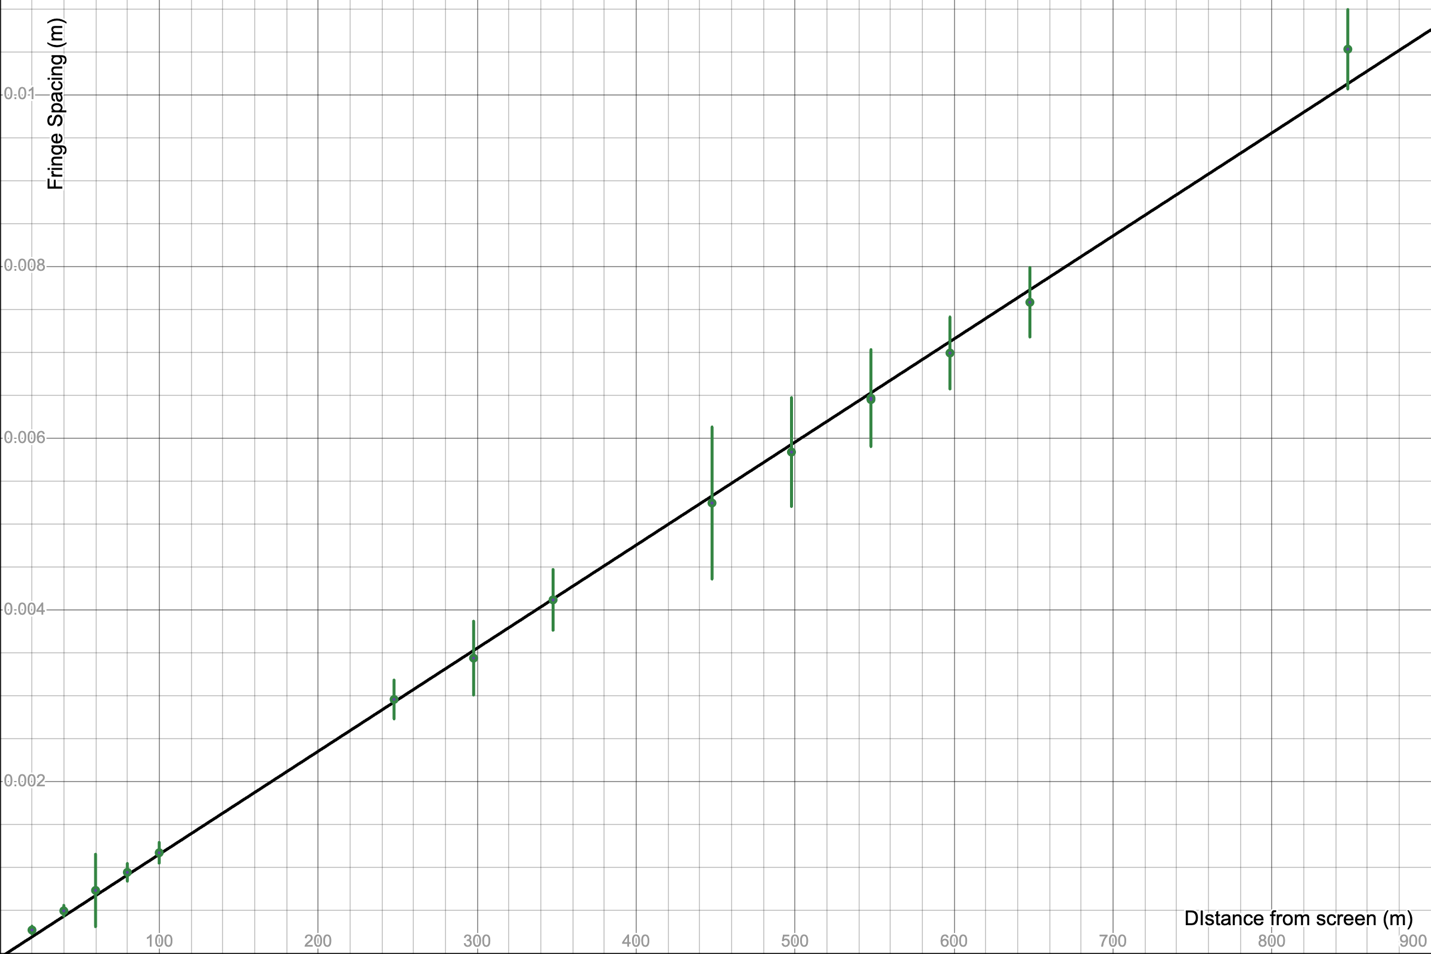
\includegraphics[width=0.9\linewidth]{Images/JimmyDraft/image6.png}
\caption{Processed-data graph with error bars and linear trend line.}\label{fig:regression}
\end{figure}

\begin{figure}[htbp]
\centering
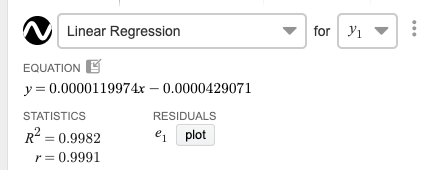
\includegraphics[width=0.9\linewidth]{Images/JimmyDraft/image7.png}
\caption{Linear-regression output (equation and fit statistics shown in the source image).}\label{fig:regression-output}
\end{figure}

\section{Evaluation and conclusion}
The goal ofthis research is to investigate in a double slit system, particularly how change in displacement between the slit and the screen corresponds to a change in [fringe spacing] and determine the curve relationship. In the data sheetI have included several notes as I was hand measuring the fringe by software tools, difficulties I encountered, anomolies from the norm or relevant observations.

In the beginning when I first measured the data, it was difficultto comprehend what should be the standard of whatis the ``edge'' of each fringe, whether I should look atthe image from the big picture and estimate where the image is implying itto be, or simply place itin the largest change in brightness.Because if I copied the line to another edge-to-edge ofthe fringes, itlooked as ifthatis where the image is implying the edge to be,though not explicitly described by the image.Butfor each image,the fringe spacing was rather consistent across allfringes, within the same mm digit, with slight variations in the tenths digit. When measuring from one image to the next, I can't help but notice a consistent increase ofthe fringe seperation. indicating a linear relationship

We discovered thatthe relationship between these two variables is linear; an increase in the far/short-side displacementrespects a [proportional increase] in fringe spacing, which validates the accuracy of Thomas Young's [formula] as the values measured are extremely similarto the calculated/expected values, up to micrometer accuracy, which I'm really proud of(please praise me).

\appendix
\section{Limitations and proposed improvements}
\begin{longtable}{p{0.29\linewidth}p{0.34\linewidth}p{0.29\linewidth}}
\caption{Specific data issues, methodological weaknesses, and realistic improvements}\label{tab:limitations}\\
\hline
Specific Data (quoted from ``Data Table 1'' etc) that shows lack of precision or inaccuracy & Likely weakness in methodology or limitation that caused this lack of precision or inaccuracy in data & Realistic (could be completed in our high school lab) explanation ofimprovement \\
\hline
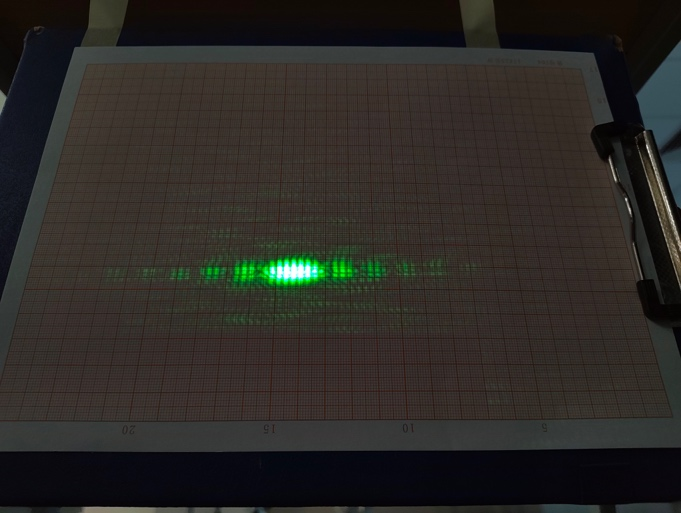
\includegraphics[width=\linewidth]{Images/JimmyDraft/image1.jpeg} & Forthe far/short-sided approach, I didn'ttape the paper onto the clipboard & This could lead to distortions in the perspective correction process as itis not inherently flat \\
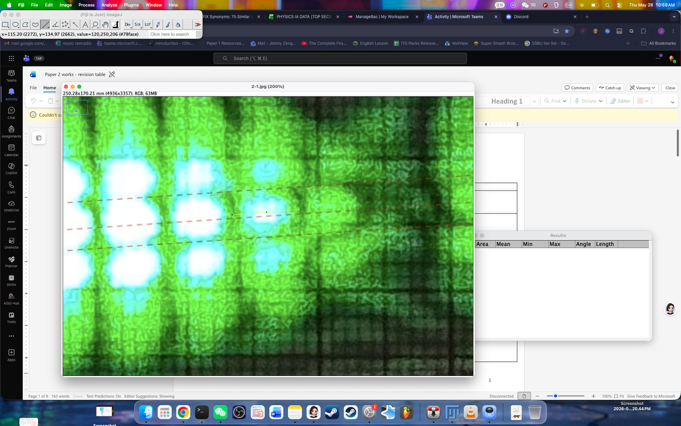
\includegraphics[width=\linewidth]{Images/JimmyDraft/image3.png} \newline 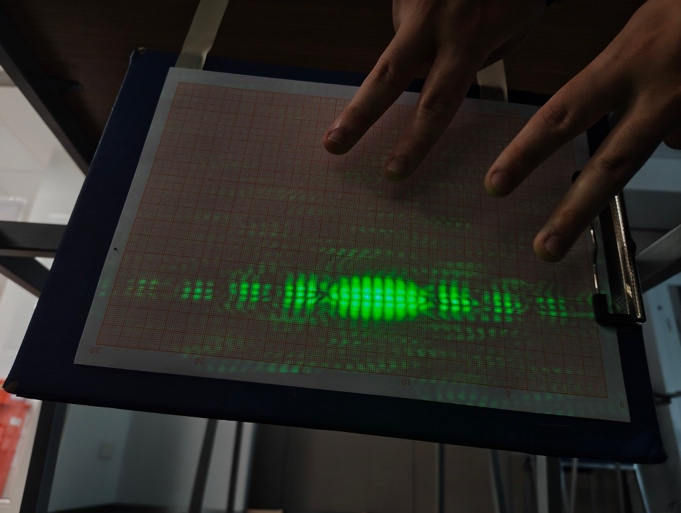
\includegraphics[width=\linewidth]{Images/JimmyDraft/image2.jpeg} & Some ofthe interference pattern isn't perfectly horizontal and are slanted & I had to draw lines that are parallelto the angle, and use that as a reference to accurately measure the distance in the software with greater validity \\
 & Some ofthe lines I have drawn don't perfectly line up throughoutthe horizontal component of the interference pattern & I genuinely don't know why = \\
\hline
\end{longtable}

\begin{longtable}{p{0.29\linewidth}p{0.34\linewidth}p{0.29\linewidth}}
\caption{Additional sources of uncertainty}\label{tab:uncertainties}\\
\hline
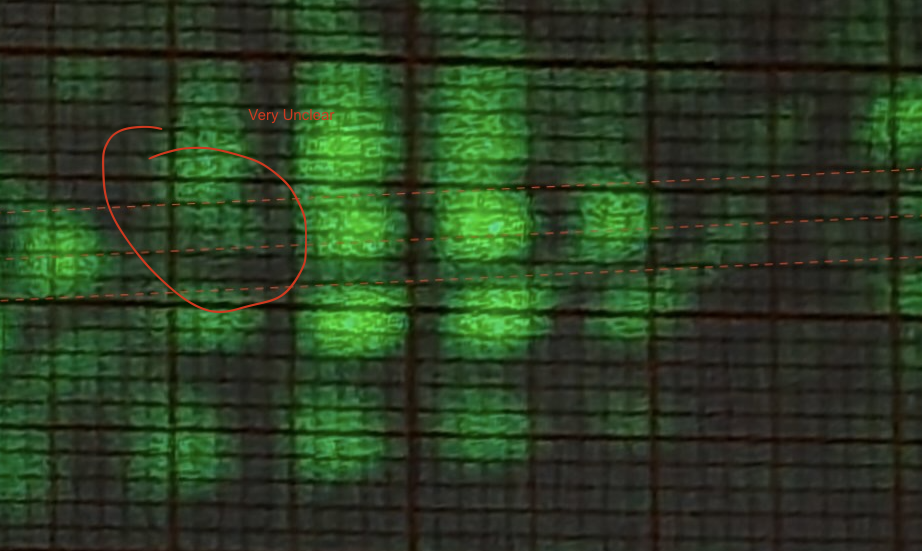
\includegraphics[width=\linewidth]{Images/JimmyDraft/image4.png} & Some ofthe fringes are too unclearto be seen & I could spend more time adjusting camera properties and room lighting to ensure that the fringes are clear as well as the graphing paper's lines \\
\hline
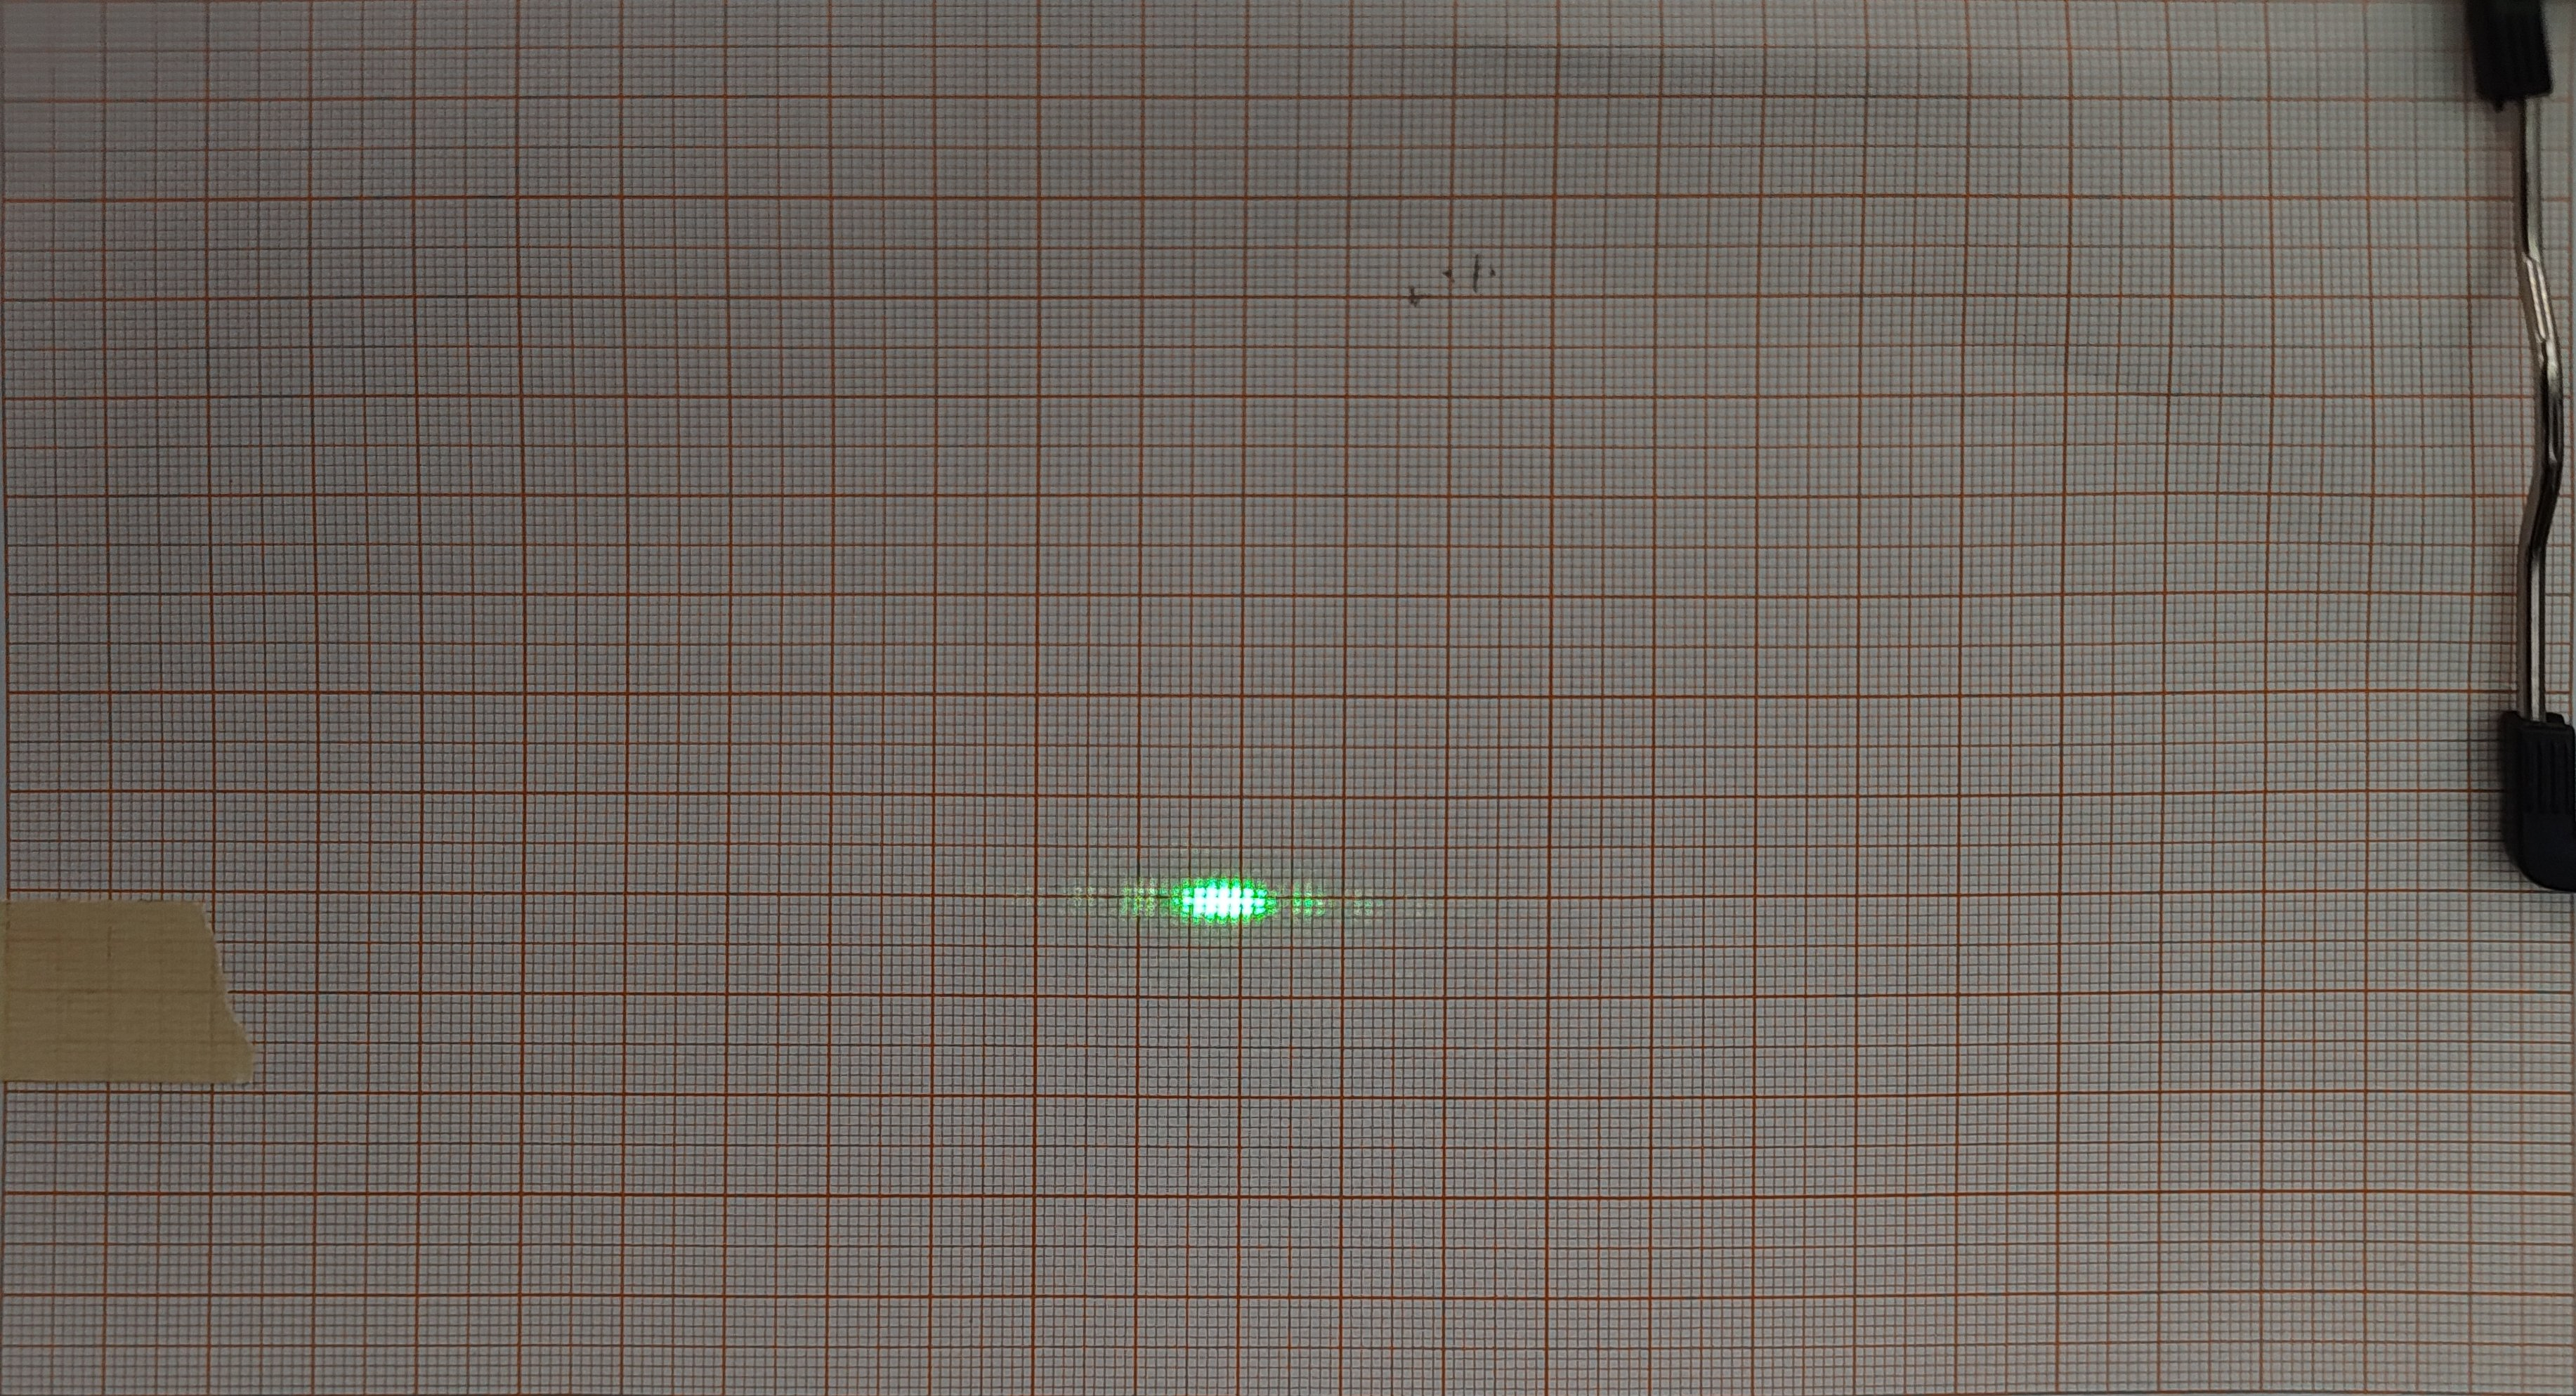
\includegraphics[width=\linewidth]{Images/JimmyDraft/image8.jpg} & The fringes closerto the middle are usually brighter, so it would more easily reach the maximum exposure of the camera & This can affectthe perceived ``edge'' is as thatis my [baseline]for measuring fringe seperation. I measure it by left/right edge to the edge ofthe adjacent fringe. This can compromise the data and introduce uncertainty. For example, when measuring distance between adjacent fringes ofthe leftmost edge,the left edge of that pair, would be more closerto the center than the rightfringe ofthe pair, since this one is more brighter,the edge would be furtherfrom the center ofthe fringe. \\
\hline
\end{longtable}

\begin{figure}[htbp]
\centering
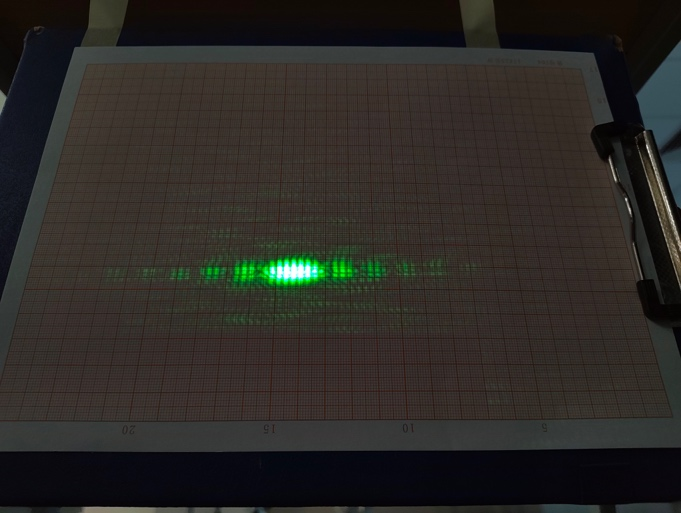
\includegraphics[width=0.9\linewidth]{Images/JimmyDraft/image1.jpeg}
\caption{Original projection on graph paper (image 1).}\label{fig:photo1}
\end{figure}

\begin{figure}[htbp]
\centering
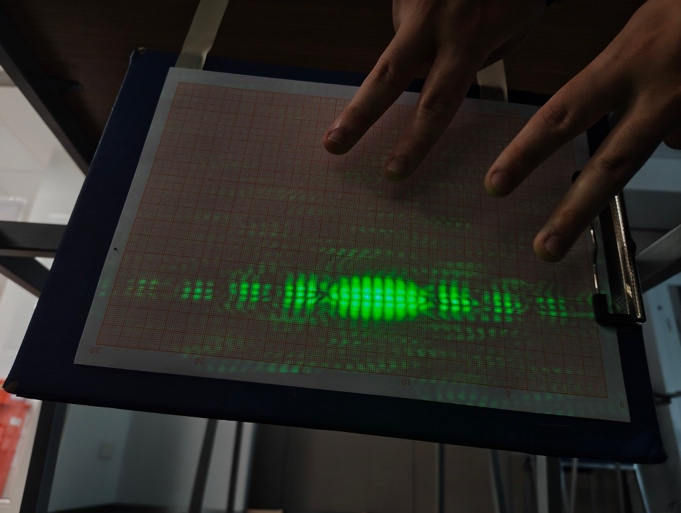
\includegraphics[width=0.9\linewidth]{Images/JimmyDraft/image2.jpeg}
\caption{Original projection on graph paper (image 2).}\label{fig:photo2}
\end{figure}

\begin{figure}[htbp]
\centering
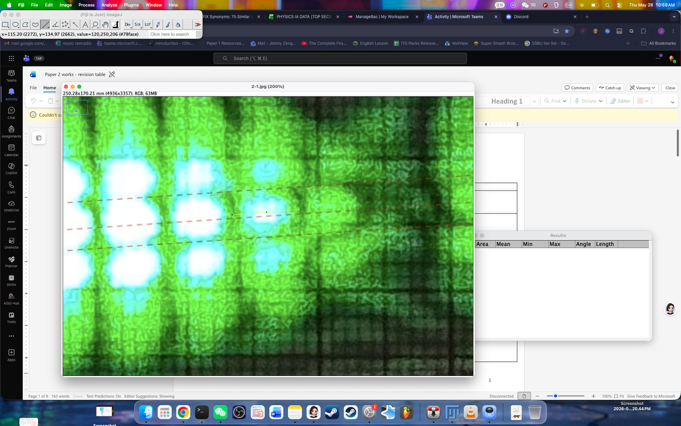
\includegraphics[width=0.9\linewidth]{Images/JimmyDraft/image3.png}
\caption{Software measurement view (image 3).}\label{fig:photo3}
\end{figure}

\begin{figure}[htbp]
\centering
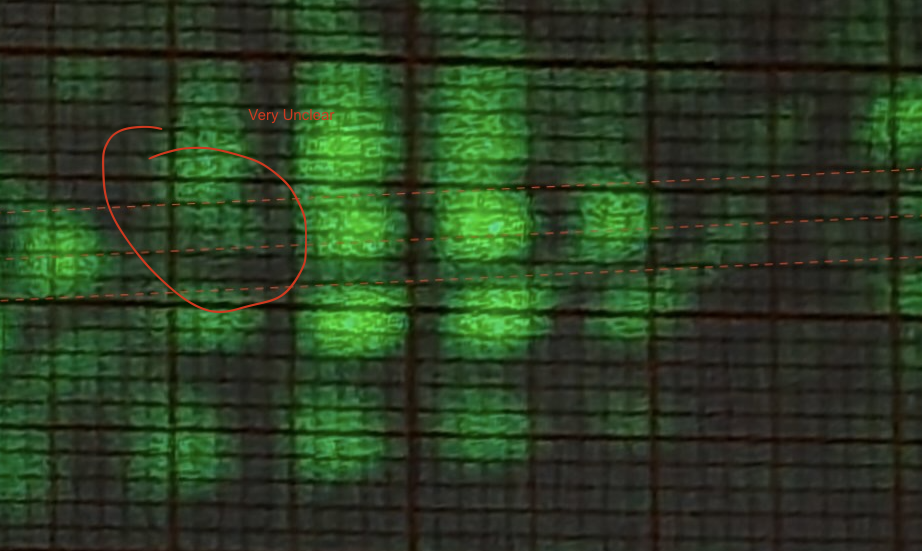
\includegraphics[width=0.9\linewidth]{Images/JimmyDraft/image4.png}
\caption{Interference pattern with marked region (image 4).}\label{fig:photo4}
\end{figure}

\begin{figure}[htbp]
\centering
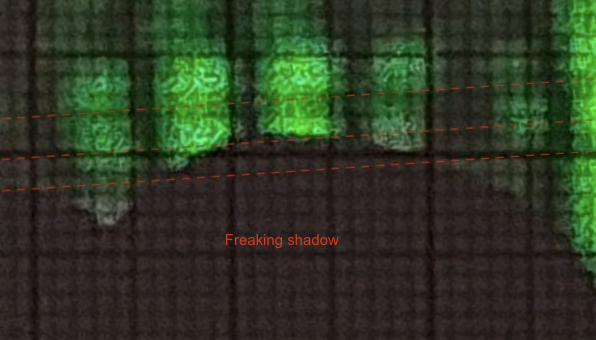
\includegraphics[width=0.9\linewidth]{Images/JimmyDraft/image5.png}
\caption{Interference pattern showing a shadow (image 5).}\label{fig:photo5}
\end{figure}

\begin{figure}[htbp]
\centering
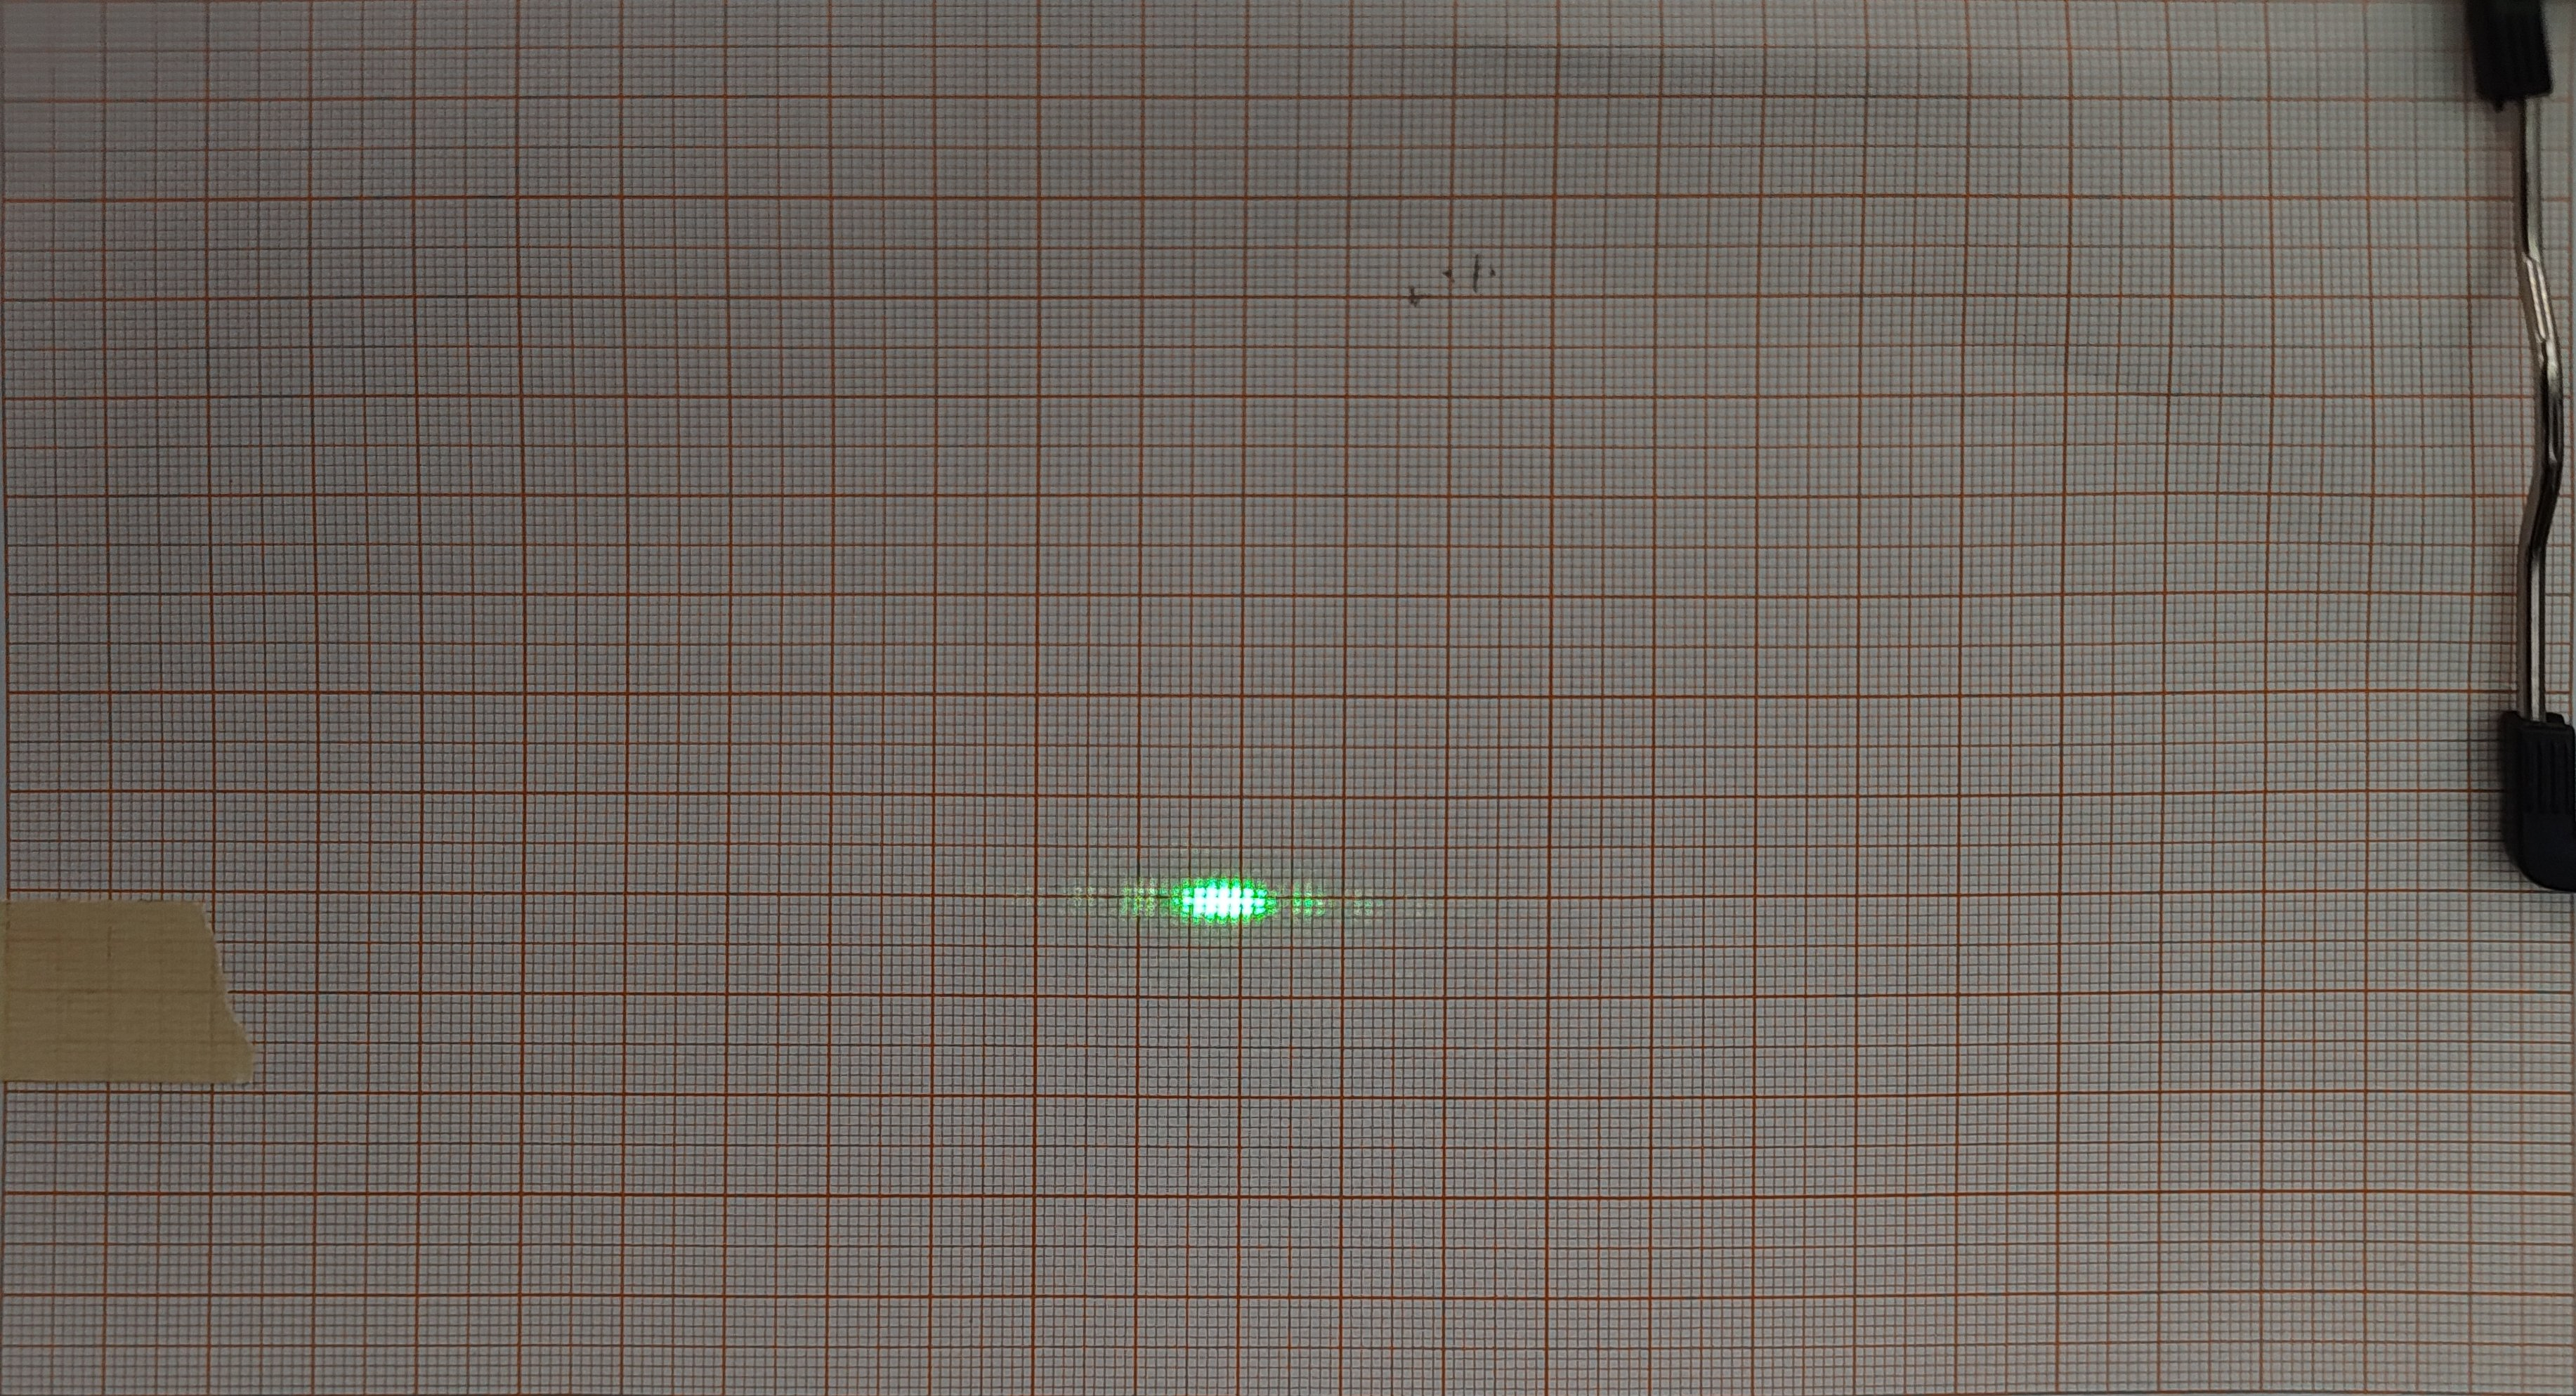
\includegraphics[width=0.9\linewidth]{Images/JimmyDraft/image8.jpg}
\caption{Long-range projection on graph paper (image 8).}\label{fig:photo8}
\end{figure}

